\documentclass{beamer}
\usetheme[
  titleformat=smallcaps,
  numbering=fraction]{metropolis}

% \usepackage{graphicx}
% \graphicspath{fig/}

\setmonofont{Fira Mono}[BoldFont={Fira Mono Medium},Scale=MatchLowercase]

\usepackage{fontawesome}

\usepackage{minted}
\usemintedstyle{vs}

\usepackage{polyglossia}
\setdefaultlanguage{swedish}

\setbeamerfont{caption}{size=\scriptsize}

\usepackage{hyperref}

\newcommand{\gittag}[1]{
  \begin{tikzpicture}[remember picture,overlay]
    \node[yshift=2ex,xshift=1em,anchor=south west] at (current page.south west) {\faicon{git}\hspace{1ex}#1};
  \end{tikzpicture}
}

\title{Modern Pythonutveckling}
\date{~}
\author{Viktor Ahlqvist}
\institute{OpKoKo 19.2\\\faicon{github}/vikahl/modern-python-development}

\begin{document}
\maketitle

{
\metroset{sectionpage=none}
\section*{Introduktion}
}

\begin{frame}{Python 2 EOL}
  \begin{columns}
    \begin{column}{0.7\linewidth}
      \begin{itemize}
        \item Python 2 EOL om 1 månad och 22 dagar
        \item \textbf{Inga} uppdateringar efter det
        \item Migrera nu!
      \end{itemize}
    \end{column}
    \begin{column}{0.3\linewidth}
      \begin{figure}
        
\includegraphics[width=\linewidth,keepaspectratio]{fig/python2eol}
        \caption{Lisa Roach, Twitter: @lisroach}
      \end{figure}
    \end{column}
  \end{columns}
\end{frame}


\begin{frame}{Förbehåll}
  \begin{itemize}
    \item "Moderna" Python-versionerna
      \begin{itemize}
        \item Python 3.6 -- 2016-12-23 (säkerhetsuppdateringar t.o.m. 2021)
        \item Python 3.7 -- 2018-06-27
        \item Python 3.8 -- 2019-10-14
      \end{itemize}
    \item Exempel fungerar på Linux/Mac, oftast också på Windows
  \end{itemize}
\end{frame}


\begin{frame}{Agenda}
  \setcounter{tocdepth}{1}
  \tableofcontents
\end{frame}

\begin{frame}{todo-extractor}
  \begin{itemize}
    \item Paket som kommer användas som exempel under föreläsningen
    \item Extraherar \textit{TODO} från kod och retunerar JSON
    \item Bra som exempelmodul, men begränsad "riktig" användbarhet
  \end{itemize}

  \faicon{github}/vikahl/todo-extractor

  \gittag{first-version}
\end{frame}

\section{Installation}

\begin{frame}{Systempython och virtualenv}
  \begin{columns}
    \begin{column}{0.7\linewidth}
      Tre korta råd
      \begin{enumerate}
        \item Undvik installation i systemets Python
        \item Använd virtuella miljöer \textit{virtual env}
        \item Ha system för flera Python versioner installerade samtidigt
      \end{enumerate}

      Tänk på att
      \begin{itemize}
        \item Kan inte se vad som installerats direkt och vad som är beroenden på dessa
        \item Kan inte på ett generellt sätt låsa beroenden i flera led
      \end{itemize}
    \end{column}
    \begin{column}{0.3\linewidth}
      \begin{figure}
        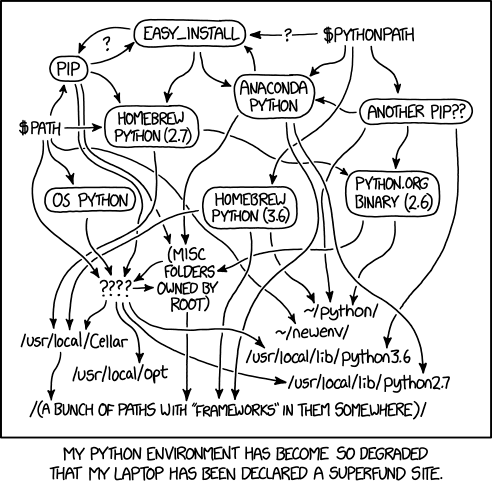
\includegraphics[width=\linewidth,keepaspectratio]{fig/python_environment}
        \caption{Randall Munroe, xkcd nr 1987}
      \end{figure}
    \end{column}
  \end{columns}
\end{frame}

\begin{frame}{Virtualenv - hantera moduler}
  \begin{itemize}
    \item Lokala paket per miljö/projekt
    \item Lätt "avinstallation" genom att ta bort mappen
    \item Skapa i skalet eller via IDE och aktiveras med aktiveringsskript\\
          \mintinline{shell-session}{python3 -m venv venv}\\
  \end{itemize}

  Glöm inte ignorera mappen i Git!
\end{frame}

\begin{frame}{pyenv - hantera versioner}
  \begin{itemize}
    \item Olika Python-version per projekt
    \item Installera versioner oberoende av systemets pakethanterare
    \item Automatisk aktivering i specifika mappar med \texttt{.python-version} filer
    \item Installera med plugins för virtualenv-stöd
  \end{itemize}

  \vfill

  \begin{figure}
    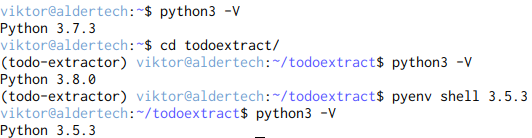
\includegraphics[width=0.8\linewidth,keepaspectratio]{fig/pyenv}
  \end{figure}
\end{frame}

\begin{frame}{pipx - hantera "binärer"}
  \begin{itemize}
    \item Isolerar Python program i separata venv
    \item Kan både installera och köra direkt
    \item Enkel uppdatering av allt installerat \mintinline{shell-session}{pipx upgrade-all}
    \item \emph{Kan ha flera versioner av samma program, men måste då manuellt symlänka}
  \end{itemize}

  Installera med \mintinline{shell-session}{pip3 install pipx}

  Bör vara \emph{den enda} paketet som är installerat i systemets Python.
\end{frame}

\begin{frame}{pipenv}
  \begin{itemize}
    \item Hanterar både beroenden och virtualenv
    \item Låser beroenden i alla led med \textit{Pipfile} och \textit{Pipfile.lock}
  \end{itemize}

  Verkade lovande, men har tappat fart och orsakar lika många problem som det löser.
\end{frame}

\section{Verktyg och kod-kvalitet}

\begin{frame}{Linters}
    \begin{itemize}
      \item Program som analyserar koden för potentiella fel
      \item PEP\,8 -- \textit{Style guide for Python code}
    \end{itemize}
\end{frame}

\begin{frame}[fragile]{Linters : Pylint}
  \begin{columns}
    \begin{column}{0.6\linewidth}
      \begin{itemize}
        \item Stilfel, syntaxfel, docstrings
        \item Statisk analys
        \item Gnällig, men fångar mycket
        \item Kräver nästan alltid konfig.
        \item Har plugins
      \end{itemize}
    \end{column}

    \begin{column}{0.4\linewidth}
      {\ttfamily\tiny
        C0326: No space allowed around keyword argument assignment\\
        C0114: Missing module docstring\\
        W0102: Dangerous default value [] as argument\\
        C0116: Missing function or method docstring\\
        E0602: Undefined variable 'my\_list'\\
        Your code has been rated at -12.50/10
      }

      \begin{minted}[fontsize=\footnotesize,autogobble]{python}
        def add_2(arg = []):
          arg.append(2)
          print(arg)
          return my_list
      \end{minted}
    \end{column}
  \end{columns}
\end{frame}

\begin{frame}[fragile]{Linters : Flake8}
  \begin{columns}
    \begin{column}{0.6\linewidth}
      \begin{itemize}
        \item Mindre gnällig
        \item Lätt att bara slänga in ett projekt
        \item Hittar mycket, men inte lika mycket
        \item Har också plugins
      \end{itemize}
    \end{column}
    \begin{column}{0.4\linewidth}
      {\ttfamily\tiny
        E251 unexpected spaces around keyword / parameter equals\\
        F821 undefined name 'my\_list'
      }

      \begin{minted}[fontsize=\footnotesize,autogobble]{python}
        def add_2(arg = []):
          arg.append(2)
          print(arg)
          return my_list
      \end{minted}
    \end{column}
  \end{columns}
\end{frame}

\begin{frame}[fragile]{Linters : Bandit}
  \begin{itemize}
    \item Söker efter säkerhetsbrister och bedömer allvarlighet och tillförlitlighet
    \item Söker både i koden och i inkluderade paket
  \end{itemize}

  \begin{minted}[fontsize=\footnotesize,autogobble]{shell-session}
    >> Issue: [B502:ssl_with_bad_version] ssl.wrap_socket call with
    insecure SSL/TLS protocol version identified, security issue.
       Severity: High   Confidence: High
       Location: ./ssl-insecure-version.py:4
       More Info: https://bandit.readthedocs.io/en/latest/plugins/b502…
    3
    4	ssl.wrap_socket(ssl_version=ssl.PROTOCOL_SSLv2)
    5	SSL.Context(method=SSL.SSLv2_METHOD)
  \end{minted}
\end{frame}

\begin{frame}{Autoformaterare : Black}
  \begin{itemize}
    \item Formatterar koden automatiskt
    \item Black -- \textit{The uncompromising code formatter}
      \begin{itemize}
        \item radlängd
        \item normalisering av citattecken
      \end{itemize}
    \item Garanterar samma exekvering av koden innan/efter
    \item Finns alternativ: \textsc{yapf}, autoformatter
  \end{itemize}

  Mitt råd: Välj Black och fokusera på affärsnytta istället
  \gittag{black}
\end{frame}

\begin{frame}[standout]{Linter och autoformatterare}
  Kör linters och autoformatterare vid PR och kräv att de ska gå igenom innan merge
\end{frame}

% \begin{frame}{Konfigurationsfiler}
%   \begin{itemize}
%       \item Traditionellt sett många olika
%       \item PEP\,518 -- {\small\textit{Specifying minimum build system requirements for Python projects}}
%       \item \texttt{pyproject.toml}, \textsc{toml}-format
%       \item Andra verktyg kan också använda den här filen men alla stödjer ännu inte denna.
%   \end{itemize}
% \end{frame}

\section{Type hinting}

\begin{frame}{Type hinting och type annotations}
  \begin{itemize}
    \item Python är fortfarande dynamiskt typat
    \item Underlättar och dokumenterar för utvecklare och IDE
    \item[]
    \item \mintinline{python}{def prepare_plot(value: int, unit: str) -> dict}
    \item Statisk typkontroll med MyPy
  \end{itemize}

  \gittag{type-hint}
\end{frame}

\begin{frame}{Typing modulen}
  \begin{itemize}
    \item \emph{typing} modulen ger fler möjligheter
    \item \mintinline{python}{typing.Union[str, int]}
    \item \mintinline{python}{typing.List[str]}
    \item \mintinline{python}{typing.Dict[str, set]}
    \item \mintinline{python}{typing.Iterable}
    \item \mintinline{python}{typing.Any}
    \item …
    \item Klasser är också typer
    \item Använd strängar för att annotera om typen inte är tillgänglig
  \end{itemize}
\end{frame}

\begin{frame}[fragile]{Nytt i 3.8}
  \begin{itemize}
    \item \mintinline{python}{Literal} definerar unika värden\\
      {\small\mintinline{python}{def print_length(length, unit=typing.Literal["m", "ft"])}}
    \item[]
    \item \mintinline{python}{Final} för värden som inte \emph{bör} defineras om\\
     \mintinline{python}{user_id: typing.Final[int] = 24}
    \item \mintinline{python}{@typing.final} för klasser och metoder som inte \emph{bör} ärvas/ändras av subklasser
  \end{itemize}
\end{frame}

\begin{frame}[fragile]{Nytt i 3.8 : TypedDict : PEP\,589}

  \begin{minted}[fontsize=\small]{python}
    class OpKoKo(typing.TypedDict):
      edition: str
      start_date: datetime.date

    current = OpKoKo(edition="19.2", date=datetime.date(2019, 11, 8)
    # …
    def printable_program(current: OpKoKo) -> str:
  \end{minted}

  \begin{itemize}
    \item Bättre kontroll av typer i en dict
    \item Objektet blir en vanlig dict
    \item Jämför: named tuple eller dataclasses
  \end{itemize}
\end{frame}

\begin{frame}[fragile]{Nytt i 3.8 : Protocols : PEP\,544}
  \begin{itemize}
    \item Static ducktyping
    \item Specifierar metoder/attribut objektet \emph{ska} ha
  \end{itemize}

  \begin{minted}[fontsize=\small,autogobble]{python}
    class ChessPiece(typing.Protocol):
      name: str
      def move(self) -> None:
        pass

    def play(piece: ChessPiece, x: int, y: int) -> None:
      piece.move(x, y)
  \end{minted}
\end{frame}

\section{Testing}

\begin{frame}{Pytest}
  \begin{itemize}
    \item Fantastiskt testramverk, bättre än Unittest från standardbiblioteket
    \item Läs Brian Okkens \emph{Python Testing with pytest} (Pragmatic bookshelf)
    \item Fixturer, plugins, rena asserts, …
    \item \mintinline{python}{assert data is not None}
  \end{itemize}
  \gittag{pytest}
\end{frame}

\begin{frame}{Testtäckning med coverage}
  \begin{itemize}
    \item Plugin till pytest: \mintinline{shell-session}{pytest --cov=todo-extractor}
    \item Mäter testtäckning
    \item Genererar rapporter för människor och maskiner\\
          \textsc{html}, \textsc{xml}, …
  \end{itemize}

  \vfill
  {\small\ttfamily
    Name                Stmts   Miss  Cover\\
    ---------------------------------------\\
    todo\_extractor.py      22      7    68%
  }
\end{frame}

\section{Paketera som modul}

\begin{frame}{Paketera som modul}
  \begin{itemize}
    \item Finns många sätt men jag rekommenderar Flit
    \item Starta med \mintinline{shell-session}{flit init}
    \item Konfigureras i \texttt{pyproject.toml}\\
      PEP\,518 -- {\small\textit{Specifying minimum build system requirements for Python projects}}
  \end{itemize}
  \gittag{flit-init}
\end{frame}

\begin{frame}{Paketera som modul}
  \begin{itemize}
    \item Stödjer inte \texttt{requirements.txt} → flytta beroenden
    \item Installera med symlänk/\texttt{pth}-filer för \textsc{tdd}
  \end{itemize}
  \gittag{flit-full}
\end{frame}

\begin{frame}[fragile]{Publicera modulen}
  \begin{itemize}
    \item Testa mot \url{test.pypi.org}
    \item Konfigurera egna servrar i \texttt{~/.pypirc}
    \item \mintinline{shell-session}{flit --repository testpypi publish}
  \end{itemize}

  \vfill

  Installera modulen med \mintinline{shell-session}{pipx install todo-extractor}

  \gittag{install-module}
\end{frame}

\section{Automatisera tester}

\begin{frame}{Automatisera med Pre-commit}
  \begin{itemize}
    \item Ramverk för att hantera git pre-commit hooks
    \item Skrivet i Python, men inte bara för Python
    \item Konfigureras med \texttt{.pre-commit} \textsc{yaml} fil
    \item Måste manuellt installeras, ersätter inte \textsc{ci}
    \item Kör linters, autoformattera JSON, …
  \end{itemize}
  \gittag{pre-commit}
\end{frame}

% \begin{frame}[fragile]{Exempel på konfiguration}
%   \begin{minted}{yaml}
%     repos:
%     - repo: https://github.com/pre-commit/pre-commit-hooks
%       rev: v2.3.0
%       hooks:
%         - id: pretty-format-json
%         - id: check-json
%     - repo: https://github.com/psf/black
%       rev: stable
%       hooks:
%       - id: black
%     - repo: https://github.com/pre-commit/mirrors-pylint
%       rev: master
%       hooks:
%       -  id: pylint
%   \end{minted}
% \end{frame}


\begin{frame}{tox}
  \begin{itemize}
    \item Automatisera tester med definerade testfall
    \item Unika virtualenv för tester -- skilj från utvecklingsvenv
    \item Möjliggör test i flera Python-versioner
    \item Passar utmärkt att köra i \textsc{ci}
  \end{itemize}

  \gittag{tox}
\end{frame}

% \input{sections/090-travis}
\section{Projektmall med cookiecutter}

\begin{frame}{Projektmall med cookiecutter}
  \begin{itemize}
    \item Ramverk för att skapa projekt från Jinja2-mallar
    \item Skrivet i Python, men inte bara för Python
    \item Kan skapa upp hela mapp- och filstrukturen
  \end{itemize}

  \faicon{github}/vikahl/python-template
\end{frame}

{%
\metroset{sectionpage=none}
\section*{Avslut}
}

\begin{frame}[standout]
  Slut, frågor?

  {\small\faicon{github}/vikahl/modern-python-development}

  {\small\faicon{github}/vikahl/todo-extractor}

  {\small\faicon{github}/vikahl/python-template}
\end{frame}

\begin{frame}
  \titlepage{}
\end{frame}

\begin{frame}{Källor och inspiration}
  \begin{itemize}
    \item Python bytes (podcast)
    \item Test and code (podcast)\\
      {\small Speciellt avsnitt 80 \emph{From Python script to maintainable package} och 81 \emph{TDD with Flit}}
    \item Talk Python to me (podcast)
    \item Real Python (\url{realpython.com})
    \item \url{docs.python.org}
  \end{itemize}
\end{frame}



\end{document}
